\documentclass[10pt,a4paper]{article}
\usepackage[margin=2.1cm]{geometry}
\usepackage{amsmath,amssymb,graphicx,booktabs,caption,float,xcolor,enumitem,array}
\usepackage{tikz}
\usetikzlibrary{arrows.meta,positioning}
\usepackage[colorlinks=true,linkcolor=blue!50!black,citecolor=blue!50!black,urlcolor=blue!50!black]{hyperref}
\captionsetup{font=small,labelfont=bf}
\setlist{itemsep=1pt,topsep=3pt}
\graphicspath{{figures/}}
\definecolor{cA}{HTML}{3b75af}
\definecolor{cC}{HTML}{d1495b}
\newtheorem{result}{Result}
\newcommand{\Sus}{\mathcal S}

\title{\textbf{The fact-flow model, derived step by step}\\[2pt]
\large and a selection mechanism for the fading of persistence}
\author{Claude (theory work, \nolinkurl{analysis/theory_claude/})}
\date{Session report, 28 October 2026}

\begin{document}
\maketitle

\begin{abstract}
\noindent
This report has two parts.
\begin{itemize}
\item \textbf{Part I (Sections 1--8)} derives the four equations of the fact-flow model from the simulator's rules. For
  each equation it says what every symbol measures, which approximations turn the simulator's rule into the equation,
  and what is lost. It then derives the results built on them: the frozen-board memory, the no-communication transient,
  the reading reversal, and the persistence threshold.
\item \textbf{Part II (Sections 9--11)} reports today's work on why the controller's effect fades after the stop in
  Object Placements but not in task003. In Object Placements the controller's facts keep circulating but stop
  persuading. A selection mechanism explains the direction of this:
  \begin{itemize}
  \item agents repost facts that support their current answer;
  \item when a controller fact pushes some readers toward the wrong answer and others away, the non-$A2$ majority keeps
    recirculating the versions that push away.
  \end{itemize}
  The parameter that sets the sign of the selection was identified only after seeing the data, so it is not yet
  validated.
\end{itemize}
A note on dates: yesterday's report and blackboard notes are labelled 28 October but were written on 27 October. This
report is the real 28 October report.
\end{abstract}

\tableofcontents
\clearpage

% ======================================================================================================================
\part*{Part I. The model and its derivations}
\addcontentsline{toc}{part}{Part I. The model and its derivations}

\section{The simulator rules that the model compresses}
\label{sec:rules}
The model is a compression of Simulation 2 (code: \nolinkurl{task003_llm_free/simulation_2/simulator/sim2/}). These are
the rules that matter.
\begin{enumerate}
\item \textbf{Agents and clocks.} $N=24$ agents. Each acts at random times, at rate 1: the gaps between actions are
  exponential with mean 1.
\item \textbf{Facts.} The task world has a set of facts. Each agent starts with one of its own (``native'') facts. The
  controller has a pool of facts selected to support the wrong answer $A2$. All facts are true.
\item \textbf{The board.}
  \begin{itemize}
  \item Posts are never deleted; the board is ``persistent''.
  \item When an agent acts, it looks only at the $W=48$ most recent posts, excluding its own. So its view is a
    \emph{sliding window}: each new post pushes the oldest one out of view.
  \item It reads $q$ of these posts, chosen at random without replacement.
  \end{itemize}
\item \textbf{Memory and forgetting.} Each fact an agent remembers (its \emph{active} facts) gets a random lifetime,
  exponential with rate $\gamma=-\ln\rho$. Reading the fact again starts a fresh lifetime. So $\rho$ is the chance
  that a remembered fact survives one time unit without being read again: $e^{-\gamma}=\rho$.
\item \textbf{Vote.} The agent computes the exact posterior probability of each of the three answers from its active
  facts. It then votes by \emph{probability matching}: it votes $A2$ with probability $P(A2\mid\text{active facts})$.
\item \textbf{Post.} The agent posts one fact that \emph{supports its vote in context}: removing it from the agent's
  memory would lower the probability of the answer it voted for. It prefers facts it did not just read. If no fact
  supports the vote, it may post nothing.
\item \textbf{Controller.} Until $T=30$, the controller posts at rate $\lambda_0=1$. It reads part of the board and
  posts the pool facts that most raise $P(A2)$ given what it read. After $T$ it is silent.
\end{enumerate}
The controller's effect is measured against a \emph{silent arm}: the same swarm with no controller. $G$ is the difference
in the share of $A2$ votes between the controlled and silent arms at $T$; $\delta(t)$ is the same difference after $T$.

% ======================================================================================================================
\section{Notation, and what ``mean field'' means here}
\label{sec:notation}

\begin{table}[h]
\centering\small
\caption{\textbf{Every symbol of the model.} ``Class'' means one of two kinds of fact: $A$ (the agents' own) or $C$
(the controller's).}
\label{tab:notation}
\begin{tabular}{@{}l p{0.72\linewidth}@{}}\toprule
symbol & meaning\\\midrule
$\alpha\in\{A,C\}$ & fact class: $A$ = native facts (initially spread one per agent), $C$ = controller facts\\
$F_\alpha$ & number of distinct facts in class $\alpha$ ($F_A=16$, $F_C=4$); facts of one class are treated as identical\\
$m_\alpha(t)$ & chance that a given agent remembers a given fact of class $\alpha$\\
$M_\alpha=F_\alpha m_\alpha$ & expected number of class-$\alpha$ facts an agent remembers\\
$b_\alpha(t)$ & share of the readable board (last $W$ posts) carrying a class-$\alpha$ fact; $1-b_A-b_C$ is background\\
$q$ & posts read per action\\
$\rho,\ \gamma=-\ln\rho$ & memory retention per time unit, and the matching forgetting rate\\
$r_\alpha$ & chance that one action brings a given class-$\alpha$ fact into memory (Eq.~\ref{eq:r})\\
$N,\ W$ & number of agents (24) and window length (48 posts)\\
$\lambda(t),\ u_\alpha$ & controller posting rate ($\lambda_0$ until $T$, then 0), and the class of its posts ($u_C=1,u_A=0$)\\
$x$ & log-odds of an $A2$ vote: $x=\ln[P(A2)/(1-P(A2))]$\\
$h_0$ & log-odds of $A2$ before any fact is known ($\ln\tfrac12$: prior $P(A2)=1/3$)\\
$\beta_C,\ \beta_A$ & evidence per fact: how much one controller fact raises, or one own fact lowers, the log-odds $x$\\
$\sigma(x)$ & the logistic function $1/(1+e^{-x})$, which turns log-odds into a probability\\
$\Phi_2$ & probability that an agent votes $A2$; $\Phi_2=\sigma(x)$\\
$\kappa_\alpha,\ \kappa_0$ & posting propensity per held fact of class $\alpha$, and the weight of a background post\\
$\varepsilon$ & share of reposting that does not depend on the agent's vote (Sec.~\ref{sec:eq4})\\
$g_\alpha$ & chance that a held class-$\alpha$ fact is eligible for posting, given the vote (Eq.~\ref{eq:g})\\
$w_\alpha$ & posting weight of class $\alpha$ for an agent: $\kappa_\alpha M_\alpha g_\alpha$\\
$S_\alpha$ & share of new agent posts that carry a class-$\alpha$ fact (Eq.~\ref{eq:4})\\
$G,\ D,\ \delta(t)$ & controller effect at $T$; its change with reading $D=G(q_2)-G(q_1)$; effect after the stop\\
$\Sus(t)$ & population susceptibility to the controller facts encountered (Sec.~\ref{sec:sus}). Written
calligraphic to avoid confusion with $S_\alpha$; yesterday's report used plain $S(t)$\\\bottomrule
\end{tabular}
\end{table}

\paragraph{The four equations.}
\begin{align}
\dot m_\alpha&=(1-m_\alpha)\,r_\alpha-\gamma\,m_\alpha,\qquad r_\alpha=1-\Big(1-\frac{b_\alpha}{F_\alpha}\Big)^{q},\label{eq:1}\\
\dot b_\alpha&=\frac NW\,(S_\alpha-b_\alpha)+\frac{\lambda(t)}W\,(u_\alpha-b_\alpha),\label{eq:2}\\
\Phi_2&=\sigma(x),\qquad x=h_0+\beta_C M_C-\beta_A M_A,\label{eq:3}\\
S_\alpha&=\frac{w_\alpha}{w_A+w_C+\kappa_0},\qquad w_\alpha=\kappa_\alpha M_\alpha\,g_\alpha,\qquad
g_C=\varepsilon+(1-\varepsilon)\Phi_2,\quad g_A=\varepsilon+(1-\varepsilon)(1-\Phi_2).\label{eq:4}
\end{align}
Yesterday's report wrote Eq.~\eqref{eq:4} as $S_\alpha\propto\kappa_\alpha M_\alpha g_\alpha$. The ``$\propto$''
(proportional to) hid the division by the total, which makes the shares of $A$, $C$ and background posts add up to 1.
Eq.~\eqref{eq:4} is the exact rule used in the code.

\begin{figure}[h]
\centering
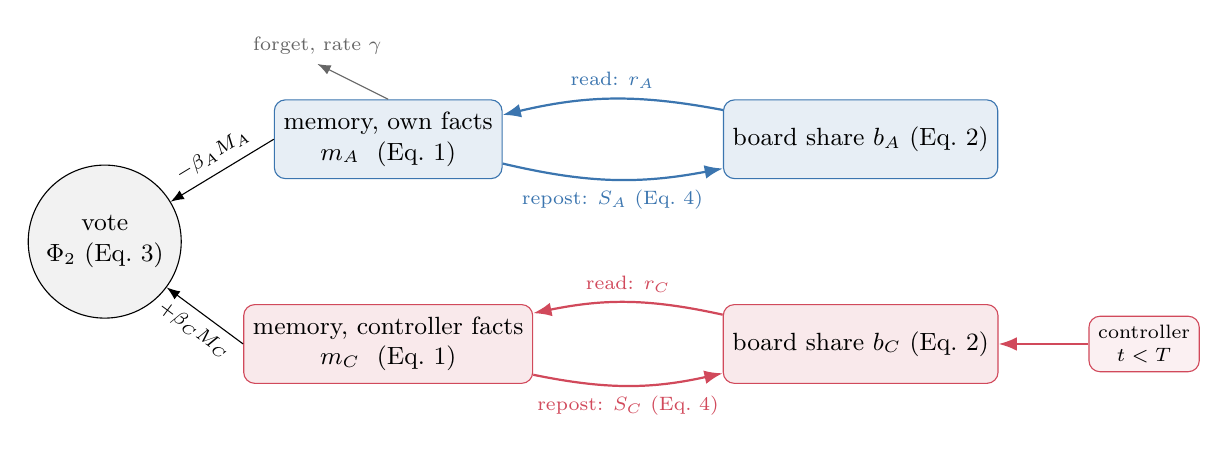
\begin{tikzpicture}[font=\small, >=Latex,
  res/.style={draw, rounded corners, minimum width=25mm, minimum height=10mm, align=center},
  lab/.style={font=\scriptsize, align=center}]
  \node[res, fill=cA!12, draw=cA] (mA) at (0,1.3) {memory, own facts\\ $m_A$ \ (Eq.~1)};
  \node[res, fill=cC!12, draw=cC] (mC) at (0,-1.3) {memory, controller facts\\ $m_C$ \ (Eq.~1)};
  \node[res, fill=cA!12, draw=cA] (bA) at (6.0,1.3) {board share $b_A$ (Eq.~2)};
  \node[res, fill=cC!12, draw=cC] (bC) at (6.0,-1.3) {board share $b_C$ (Eq.~2)};
  \node[draw, circle, fill=black!5, minimum size=12mm, align=center] (V) at (-3.6,0) {vote\\ $\Phi_2$ (Eq.~3)};
  \node[draw=cC, rounded corners, fill=cC!8, font=\scriptsize, align=center] (ctrl) at (9.6,-1.3) {controller\\ $t<T$};
  \draw[->, thick, cA] (bA) to[bend right=12] node[lab, above] {read: $r_A$} (mA);
  \draw[->, thick, cA] (mA) to[bend right=12] node[lab, below] {repost: $S_A$ (Eq.~4)} (bA);
  \draw[->, thick, cC] (bC) to[bend right=12] node[lab, above] {read: $r_C$} (mC);
  \draw[->, thick, cC] (mC) to[bend right=12] node[lab, below] {repost: $S_C$ (Eq.~4)} (bC);
  \draw[->, thick, cC] (ctrl) -- (bC);
  \draw[->] (mA.west) -- node[lab, above, sloped] {$-\beta_A M_A$} (V);
  \draw[->] (mC.west) -- node[lab, below, sloped] {$+\beta_C M_C$} (V);
  \draw[->, black!60] (mA.north) -- ++(-0.9,0.45) node[lab, above] {forget, rate $\gamma$};
\end{tikzpicture}
\caption{\textbf{Which equation does what.} Eq.~1 moves facts from the board into memory and forgets them. Eq.~2 moves
facts from memory onto the board. Eq.~3 turns memory into a vote. Eq.~4 decides what is reposted. The vote also
feeds back on reposting through the gating $g_\alpha$, whose strength is set by $\varepsilon$ (not drawn).}
\label{fig:model}
\end{figure}

\paragraph{What ``mean field'' means here.} The model replaces the swarm with one average agent and the board with
its average composition. Concretely, it makes four approximations:
\begin{enumerate}
\item \textbf{One average agent.} All agents share one $m_\alpha$. Differences between agents are lost, and so are
  correlations between facts in one memory. Facts read in the same action arrive together, so in reality they are
  remembered together more often than independence implies (the ChatGPT agent's ``co-retention'').
\item \textbf{The vote at the average.} $\Phi_2=\sigma(x(\bar M))$, the vote of an agent holding the \emph{average}
  numbers of facts, not the average of $\sigma(x(M))$ over agents. Because $\sigma$ is curved, the two differ.
\item \textbf{Deterministic shares.} $m_\alpha$ and $b_\alpha$ are smooth numbers, not counts. A class can shrink but
  never reach exactly zero, so no fact can go extinct.
\item \textbf{Interchangeable facts} within a class, read from a well-mixed board.
\end{enumerate}
\textbf{Why finite $F_\alpha$ is still mean field.} The limit that makes the equations exact is $N\to\infty$ and
$W\to\infty$ with $N/W$ and $F_\alpha$ fixed. In this limit each fact has infinitely many copies, so its share moves
smoothly and never hits zero. What the model misses is the finite number of copies per fact, about $N/F$ in memories
and $W/F$ on the board. That is exactly what the finite model restores (Sec.~\ref{sec:finite}).

% ======================================================================================================================
\section{Equation 1: memory}
\label{sec:eq1}
\paragraph{Step 1: one agent, one fact.} Let $I(t)=1$ if a given agent remembers a given fact $f$ of class $\alpha$,
and 0 otherwise. In a short time $dt$:
\begin{itemize}
\item if $I=1$, the fact is forgotten with probability $\gamma\,dt$. Its lifetime is exponential with rate $\gamma$.
  Re-reading it restarts the lifetime, but an exponential lifetime has no memory of its age, so restarting changes
  nothing.
\item if $I=0$, the agent acts with probability $dt$ (rate 1). When it acts, it picks up $f$ with probability $r_\alpha$.
\end{itemize}
Taking expectations, with $m=\mathbb E[I]$:
\begin{equation}
m(t+dt)=m(t)\,(1-\gamma\,dt)+(1-m(t))\,r_\alpha\,dt\quad\Longrightarrow\quad \dot m=(1-m)\,r_\alpha-\gamma\,m .
\end{equation}
This step is exact for one agent \emph{if} $r_\alpha$ is a fixed number. It becomes a mean-field approximation because
$r_\alpha$ depends on the board, which is random and correlated with what this agent holds; the model uses the average
board.

\paragraph{Step 2: the reading chance $r_\alpha$.} The class share $b_\alpha$ is split equally among the $F_\alpha$
interchangeable facts, so one post carries the specific fact $f$ with probability $b_\alpha/F_\alpha$. The model draws
the $q$ posts independently (with replacement):
\begin{equation}
\Pr[\text{none of the $q$ posts carries } f]=\Big(1-\frac{b_\alpha}{F_\alpha}\Big)^q
\quad\Longrightarrow\quad r_\alpha=1-\Big(1-\frac{b_\alpha}{F_\alpha}\Big)^q .\label{eq:r}
\end{equation}
The simulator draws without replacement from a window of $W$ posts. If $k=Wb_\alpha/F_\alpha$ of those posts carry $f$,
then exactly
\begin{equation}
r^{\text{exact}}_\alpha=1-\binom{W-k}{q}\Big/\binom{W}{q}.
\end{equation}
For $q\ll W$ the two agree. For example, with $W=48$, $q=6$ and $k=4$: $0.425$ exact against $0.407$ with replacement.

\paragraph{Three consequences.}
\begin{itemize}
\item \textbf{Frozen board.} If $b_\alpha$ is held fixed, Eq.~\eqref{eq:1} is linear, with solution
  \begin{equation}
  m_\alpha(t)=m_\alpha^*+(m_\alpha(0)-m_\alpha^*)\,e^{-(r_\alpha+\gamma)t},\qquad m_\alpha^*=\frac{r_\alpha}{r_\alpha+\gamma}.\label{eq:frozen}
  \end{equation}
  Memory settles in a time $1/(r+\gamma)$, at a level set by the balance of reading against forgetting. A frozen board
  that carries the controller's facts keeps the effect for ever (the observed ``frozen board keeps it'').
\item \textbf{Short memory} ($\gamma$ large): $m^*\approx r/\gamma$, small and proportional to reading.
\item \textbf{Long memory} ($\gamma\to0$): $m^*\to1$. Agents eventually hold everything they ever see.
\end{itemize}

% ======================================================================================================================
\section{Equation 2: the board}
\label{sec:eq2}
\paragraph{Step 1: what one post does.} Let $n_\alpha$ be the number of class-$\alpha$ posts in the window of the $W$ most
recent posts, so that $b_\alpha=n_\alpha/W$. Each new post enters the window and pushes the oldest one out:
\begin{equation}
n_\alpha\ \to\ n_\alpha+\mathbf 1[\text{new post is }\alpha]-\mathbf 1[\text{oldest post is }\alpha].
\end{equation}

\paragraph{Step 2: rates.} Agents post at total rate $N$, assuming every action produces a post. Each post carries class
$\alpha$ with probability $S_\alpha$ (Eq.~\ref{eq:4}). The controller posts at rate $\lambda$, always class $C$
($u_C=1$). Taking expectations,
\begin{equation}
\frac{d\,\mathbb E[n_\alpha]}{dt}=N S_\alpha+\lambda u_\alpha-(N+\lambda)\,\Pr[\text{oldest post is }\alpha].
\end{equation}

\paragraph{Step 3: the mean-field step.} The model sets $\Pr[\text{oldest is }\alpha]\approx b_\alpha$: the post leaving
is like an average post. Dividing by $W$ gives Eq.~\eqref{eq:2}.

\paragraph{What this step really assumes.} In a true sliding window, the oldest post is the one made $W$ posts ago, about
$\tau=W/(N+\lambda)$ time units earlier. So exactly,
$\Pr[\text{oldest is }\alpha]=S_\alpha(t-\tau)$, a delayed copy of what was posted then. Replacing it with $b_\alpha(t)$
turns the delay into exponential forgetting: the solution of Eq.~\eqref{eq:2} without the controller is
\begin{equation}
b_\alpha(t)=\int_0^\infty \frac NW\,e^{-Ns/W}\,S_\alpha(t-s)\,ds .
\end{equation}
\textbf{The model's board is therefore a continuously fading board:} every post's weight decays exponentially with age,
with mean lifetime $W/N=2$ time units. The simulator's window instead gives every post equal weight until it is $W$
posts old, and then zero (Fig.~\ref{fig:kernels}). The two have the same turnover rate, and in the mean field they give
the same steady states and the same growth thresholds. They differ in three ways:
\begin{enumerate}
\item \textbf{When the posting rate changes.} A count-based window slows down when agents post less, for instance when
  they abstain. A time-based fade does not.
\item \textbf{Fluctuations.} In a sliding window every post stays for the same number of posts. Under exponential fading,
  lifetimes are random: some posts vanish fast and others stay long. That raises the variance of the number of times a
  post is read, which matters in the finite model (Sec.~\ref{sec:finite}).
\item \textbf{Abstentions.} The rate $N/W$ assumes every action produces a post. In the simulator agents sometimes post
  nothing, so its real turnover is slower.
\end{enumerate}
\begin{figure}[h]
\centering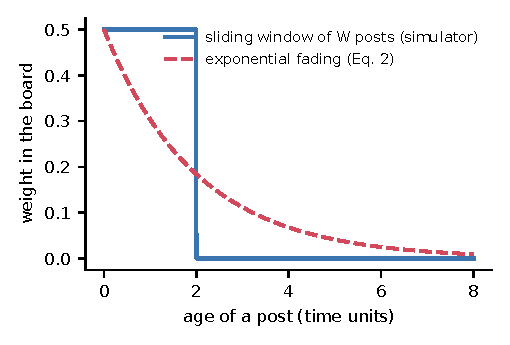
\includegraphics[width=0.48\linewidth]{fig_kernels.pdf}
\caption{\textbf{How the board remembers past posts.} The simulator's sliding window (solid) against the model's
exponential fading (dashed), with the same turnover. Eq.~\eqref{eq:2} replaces the first with the second.}
\label{fig:kernels}
\end{figure}

% ======================================================================================================================
\section{Equation 3: the vote}
\label{sec:eq3}
\paragraph{Step 1: Bayes' rule in log-odds.} Lump the two other answers together as ``not $A2$''. For a memory $M$ that
gains one more fact $f$, Bayes' rule gives
\begin{equation}
\ln\frac{P(A2\mid M\cup f)}{P(\neg A2\mid M\cup f)}=\ln\frac{P(A2\mid M)}{P(\neg A2\mid M)}
+\underbrace{\ln\frac{P(f\mid A2,M)}{P(f\mid\neg A2,M)}}_{\theta_f(M)} .\label{eq:bayes}
\end{equation}
Each fact adds its \emph{log-likelihood ratio} $\theta_f(M)$, which measures how much more likely the fact is if $A2$ is
true than if it is not, given what the agent already knows.

\paragraph{Step 2: the independence assumption.} Assume each fact's ratio does not depend on the other facts held, so
$\theta_f(M)=\theta_f$. Starting from the prior $P(A2)=1/3$, whose log-odds are $h_0=\ln\frac{1/3}{2/3}=\ln\frac12$, the
log-odds after collecting the facts in $M$ are a sum:
\begin{equation}
x(M)=h_0+\sum_{f\in M}\theta_f .
\end{equation}
This is the ``naive Bayes'' form. It is exact only if the facts are independent given the answer. On the real tasks they
are not: facts are combined into proofs, and a fact's meaning depends on the others. Yesterday's tests showed that
the same controller fact can push towards $A2$ in one context and away in another.

\paragraph{Step 3: interchangeable facts and the mean field.} Give every controller fact the same ratio $\theta=+\beta_C$
and every own fact $\theta=-\beta_A$. An agent holding $M_C$ controller facts and $M_A$ own facts then has
$x=h_0+\beta_C M_C-\beta_A M_A$. The mean field inserts the average numbers, which gives Eq.~\eqref{eq:3}.

\paragraph{Step 4: from log-odds to a vote.} $\Phi_2=\sigma(x)=1/(1+e^{-x})$ converts log-odds back into a probability.
Because the simulator votes by probability matching (rule 5), the posterior \emph{is} the vote probability, so
$\Phi_2$ is directly the expected share of $A2$ votes. (The measured effect uses each agent's last vote, which lags
slightly behind. The ChatGPT agent's model keeps this lag as $\dot v=\Phi-v$.)

\paragraph{What $\beta$ means, with numbers.} One fact multiplies the odds of $A2$ by $e^{\beta}$. With $\beta=0.5$,
that factor is $1.65$. An agent with no facts votes $A2$ with probability $\sigma(\ln\frac12)=1/3$. With two controller
facts and one own fact, $x=\ln\frac12+2(0.5)-0.5=-0.19$, so $\Phi_2=0.45$.

\paragraph{The sensitivity $\sigma'$.} How much one more fact changes the vote depends on where the agent sits:
\begin{equation}
\sigma(x+\beta)-\sigma(x)\approx\beta\,\sigma'(x),\qquad \sigma'(x)=\sigma(x)\,(1-\sigma(x)).\label{eq:sens}
\end{equation}
$\sigma'$ is largest, $1/4$, at $x=0$, the tipping point where $\Phi_2=1/2$. It falls on either side
(Fig.~\ref{fig:sigmoid}). This one fact is behind the reading reversal (Sec.~\ref{sec:reversal}).
\begin{figure}[h]
\centering
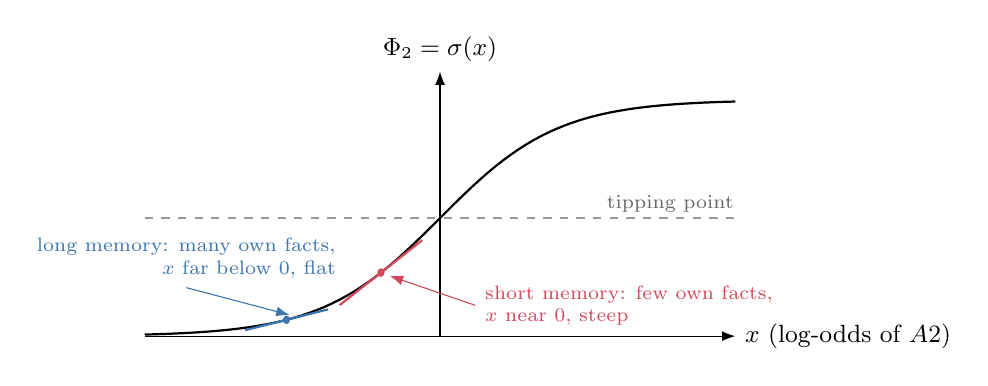
\begin{tikzpicture}[>=Latex, font=\small, xscale=0.75, yscale=3]
  \draw[->] (-5,0) -- (5,0) node[right] {$x$ (log-odds of $A2$)};
  \draw[->] (0,0) -- (0,1.12) node[above] {$\Phi_2=\sigma(x)$};
  \draw[thick, black] plot[domain=-5:5, samples=80] (\x, {1/(1+exp(-\x))});
  \draw[dashed, black!40] (-5,0.5) -- (5,0.5);
  \node[font=\scriptsize, black!60] at (3.9,0.56) {tipping point};
  \fill[cA] (-2.6,{1/(1+exp(2.6))}) circle (0.06 and 0.018);
  \fill[cC] (-1.0,{1/(1+exp(1.0))}) circle (0.06 and 0.018);
  \draw[cA, thick] (-3.3,{1/(1+exp(2.6))-0.7*0.0627}) -- (-1.9,{1/(1+exp(2.6))+0.7*0.0627});
  \draw[cC, thick] (-1.7,{1/(1+exp(1.0))-0.7*0.1966}) -- (-0.3,{1/(1+exp(1.0))+0.7*0.1966});
  \node[cA, font=\scriptsize, align=right, anchor=east] (lA) at (-1.6,0.33) {long memory: many own facts,\\ $x$ far below 0, flat};
  \draw[->, cA, thin] (lA.south) -- (-2.55,0.09);
  \node[cC, font=\scriptsize, align=left, anchor=west] (lC) at (0.6,0.13) {short memory: few own facts,\\ $x$ near 0, steep};
  \draw[->, cC, thin] (lC.west) -- (-0.85,0.255);
\end{tikzpicture}
\caption{\textbf{The vote curve and the sensitivity.} The slope $\sigma'(x)$ is how much one more fact moves the vote.
Agents who have accumulated many own facts sit far below the tipping point, where the curve is flat.}
\label{fig:sigmoid}
\end{figure}

% ======================================================================================================================
\section{Equation 4: what gets reposted}
\label{sec:eq4}
\paragraph{Step 1: one agent's choice.} At each action the agent posts one fact. The model gives each remembered fact a
weight and picks one in proportion to the weights:
\begin{itemize}
\item a remembered class-$\alpha$ fact has weight $\kappa_\alpha\,g_\alpha$;
\item a ``background'' option has weight $\kappa_0$. It stands for posts that are neither $A$ nor $C$ facts (neutral
  facts), and it keeps the board from consisting only of the two classes.
\end{itemize}
An agent holding $M_A$ own and $M_C$ controller facts therefore posts a class-$\alpha$ fact with probability
\begin{equation}
\frac{\kappa_\alpha M_\alpha g_\alpha}{\kappa_A M_A g_A+\kappa_C M_C g_C+\kappa_0}=\frac{w_\alpha}{w_A+w_C+\kappa_0}.
\end{equation}
Dividing by the total is what makes the three options' probabilities add up to 1. That is why $S_\alpha$ is
``proportional to'' $w_\alpha$ and not equal to it.

\paragraph{Step 2: the mean-field step.} $S_\alpha$ should be the \emph{average} of this ratio over agents. The model
uses the ratio of the averages instead, inserting the average $M_\alpha$. This gives Eq.~\eqref{eq:4}.

\paragraph{Step 3: the gating $g_\alpha$ and $\varepsilon$.} The simulator posts only facts that support the agent's
current vote (rule 6). The model compresses this into one number:
\begin{equation}
g_C=\varepsilon+(1-\varepsilon)\,\Phi_2,\qquad g_A=\varepsilon+(1-\varepsilon)\,(1-\Phi_2).\label{eq:g}
\end{equation}
Read it as follows. A held controller fact is eligible for posting in two ways:
\begin{itemize}
\item with probability $\varepsilon$, whatever the agent's vote;
\item otherwise, only if the agent votes $A2$, which happens with probability $\Phi_2$ under probability matching. A
  controller fact is assumed to support $A2$.
\end{itemize}
Own facts are assumed to support the other answers, so they get $1-\Phi_2$.
\begin{itemize}
\item $\varepsilon=1$: neutral reposting. The vote plays no role.
\item $\varepsilon=0$: strict gating. Only $A2$ voters repost controller facts.
\end{itemize}
In the stored simulator data, a held controller fact is eligible about 80\% of the time in task003 and 55\% in Object
Placements.

\paragraph{What Eq.~4 leaves out.} Three things:
\begin{itemize}
\item \textbf{Support in context.} In the simulator, support is measured with the agent's other facts. A controller
  fact can support a non-$A2$ vote. Part II shows that this matters.
\item \textbf{Preferring facts not just read.}
\item \textbf{Abstentions,} when no fact supports the vote.
\end{itemize}
Values ($\kappa_A=\kappa_C=1$, $\kappa_0=0.2$) were set before any run, as round numbers.

% ======================================================================================================================
\section{What follows from the four equations}
\label{sec:derived}
The parameters were fixed before any run (set ``P0''):
\begin{itemize}
\item \textbf{Taken from the simulator:} $N/W=24/48$, $W=48$, $T=30$, $h_0=\ln\frac12$.
\item \textbf{Round numbers of the right order, not measured:} $F_A=16$, $F_C=4$, $\beta_A=\beta_C=0.5$,
  $\kappa_A=\kappa_C=1$, $\kappa_0=0.2$, $\lambda_0=1$.
\end{itemize}

\subsection{No communication: a transient rise}
Switch off reading and posting at $T$. Then $r=0$ and $m_\alpha(T+s)=m_\alpha(T)e^{-\gamma s}$, so in each arm
\begin{equation}
x(s)-h_0=e^{-\gamma s}\,\big(x(T)-h_0\big).
\end{equation}
Both arms slide back to the prior, so $\delta\to0$. Differentiating $\delta=\sigma(x_c)-\sigma(x_s)$ at $s=0$:
\begin{equation}
\frac{d\delta}{ds}\Big|_{0}=-\gamma\Big[\sigma'(x_c)(x_c-h_0)-\sigma'(x_s)(x_s-h_0)\Big].
\end{equation}
This can be \emph{positive}. The silent arm is held below the prior by its own facts. As those fade, it drifts up toward
$1/3$; the controlled arm does too, but at a different rate. The model shows this at $\rho=0.75$ (0.027 rising to 0.063),
as do the simulator's symmetric setups.

\subsection{The reading reversal}
\label{sec:reversal}
Write the silent arm's log-odds as $x_s=h_0-\beta_A M_A^S$. The controller shifts the controlled arm by the \emph{net
displacement}
\begin{equation}
B=\beta_C M_C-\beta_A\big(M_A^C-M_A^S\big),\qquad x_c=x_s+B,\qquad G=\sigma(x_s+B)-\sigma(x_s).
\end{equation}
The second term of $B$ counts the agents' own facts crowded out by the controller (the ChatGPT agent's correction).
Differentiate $G$ with respect to reading $q$ and use $\partial_q x_s=-\beta_A\partial_q M_A^S$:
\begin{equation}
\partial_q G=\sigma'(x_c)\,(\partial_q x_s+\partial_q B)-\sigma'(x_s)\,\partial_q x_s
=\underbrace{\sigma'(x_c)\,\partial_q B}_{\text{exposure}}
+\underbrace{\beta_A\,\partial_q M_A^S\,\big[\sigma'(x_s)-\sigma'(x_c)\big]}_{\text{sensitivity}} .\label{eq:rev}
\end{equation}
\begin{itemize}
\item \textbf{Exposure term (positive).} Reading spreads the controller's facts.
\item \textbf{Sensitivity term (negative below the tipping point).} When $x_s<x_c<0$, $\sigma'(x_s)<\sigma'(x_c)$, and
  reading adds own facts ($\partial_q M_A^S>0$). Reading pushes the whole population down the flat part of the curve
  (Fig.~\ref{fig:sigmoid}).
\end{itemize}
Short memory keeps few own facts, so the first term wins and $D>0$. Long memory lets own facts accumulate, so the
second wins and $D<0$. For a small $B$, $\sigma'(x_c)-\sigma'(x_s)\approx\sigma''(x_s)B$ with
$\sigma''=\sigma'(1-2\sigma)$, which gives
\begin{equation}
\partial_q G\approx\sigma'(x_s)\Big[\partial_q B-(1-2\Phi_s)\,\beta_A\,B\,\partial_q M_A^S\Big].
\end{equation}
\begin{figure}[h]
\centering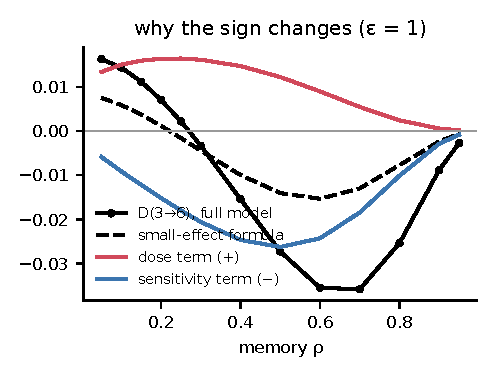
\includegraphics[width=0.48\linewidth]{fig3_dose_sensitivity.pdf}
\caption{\textbf{The two terms of Eq.~\eqref{eq:rev}} in the model (P0), with the full model's reading increment.}
\label{fig:dose}
\end{figure}

\subsection{Persistence: the growth number $\mathcal R_C$}
\label{sec:RC}
After the stop ($\lambda=0$), ask whether a small amount of controller facts grows or dies out. For small $b_C$ and
$m_C$:
\begin{itemize}
\item $r_C\approx q\,b_C/F_C$;
\item $1-m_C\approx1$;
\item $S_C\approx\kappa_C F_C m_C g_C/H$, with $H=\kappa_A M_A g_A+\kappa_0$, the posting weight of everything else.
\end{itemize}
Eqs.~\eqref{eq:1}--\eqref{eq:2} become linear:
\begin{equation}
\frac{d}{dt}\begin{pmatrix}m_C\\ b_C\end{pmatrix}=
\begin{pmatrix}-\gamma & q/F_C\\ \frac NW\,\frac{\kappa_C F_C g_C}{H} & -\frac NW\end{pmatrix}
\begin{pmatrix}m_C\\ b_C\end{pmatrix}.
\end{equation}
The trace is negative. The determinant is $\frac NW\big[\gamma-q\kappa_C g_C/H\big]$. A negative determinant means one
growing direction, so the controller's facts grow if and only if
\begin{equation}
\boxed{\ \mathcal R_C=\frac{q\,\kappa_C\,g_C}{\gamma\,H}>1\ }.\label{eq:R}
\end{equation}

\paragraph{Reading $\mathcal R_C$ as ``copies per copy''.} Follow one remembered copy of a controller fact through the
cycle:
\begin{itemize}
\item it is remembered for a mean time $1/\gamma$;
\item meanwhile its holder posts it at rate $\kappa_C g_C/H$ (its share of the holder's posting);
\item each post stays on the board for about $W/N$ time units;
\item during that time, agents act at total rate $N$, and each picks it with probability $q/W$.
\end{itemize}
New remembered copies per copy: $\frac1\gamma\cdot\frac{\kappa_C g_C}{H}\cdot\frac WN\cdot N\frac qW=\mathcal R_C$.

$N/W$ cancels: board turnover sets the speed, not the threshold. With strict gating ($\varepsilon=0$), $g_C=\Phi_2$ is
small, $\mathcal R_C\approx0.2$, and nothing persists. With neutral reposting ($\varepsilon=1$), facts keep circulating
(Fig.~\ref{fig:thr}).
\begin{figure}[h]
\centering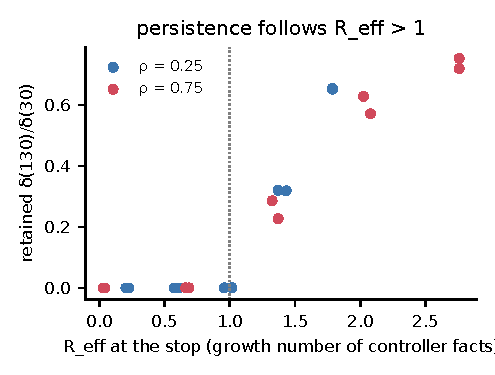
\includegraphics[width=0.44\linewidth]{fig4_threshold.pdf}
\caption{\textbf{Retained effect against the growth number} $\mathcal R_C$ in the mean-field model.}
\label{fig:thr}
\end{figure}

% ======================================================================================================================
\section{The finite model: copies per fact}
\label{sec:finite}
The finite model plays the same four rules with 24 agents and 48 whole posts, so a fact can disappear for good. The
effective finite size is not $N$ but the number of copies per fact, about $N/F$ and $W/F$: 1.5 and 3 for own facts, 6
and 12 for controller facts. Each fact behaves like a near-critical branching lineage ($\mathcal R_f\approx1$). The
ChatGPT agent's exact result for a critical lineage started from $c$ copies is
\begin{equation}
\Pr[\text{extinct by }t]=\Big(\frac{t}{1+t}\Big)^{c},
\end{equation}
while the mean number of copies stays constant. Few copies per fact means fast extinction, even though the average is
unchanged. So the swarm's widely spread facts die out while the controller's concentrated ones survive. That raises the
effect fourfold, to the simulator's level.

\section{Susceptibility}
\label{sec:sus}
Equation~\eqref{eq:bayes} gives the exact effect on $P(A2)$ of adding fact $f$ to memory $M$:
$\Delta P=\sigma(x(M)+\theta_f(M))-\sigma(x(M))$. The population's susceptibility is the average over memories $M$ in
the population ($\mu_t$) and over the controller facts $f$ actually on the board ($w_t$):
\begin{equation}
\Sus(t)=\mathbb E_{M\sim\mu_t}\,\mathbb E_{f\sim w_t}\big[\sigma(x(M)+\theta_f(M))-\sigma(x(M))\big].
\end{equation}
It is an \emph{observable}, measured on stored memories with the exact posterior. As the ChatGPT agent pointed out, it is
not yet a state variable with its own equation. Yesterday it fell 36--80\% in Object Placements no-proof and stayed flat
in task003. Part II asks why.

% ======================================================================================================================
\part*{Part II. Today: why persistence fades in Object Placements}
\addcontentsline{toc}{part}{Part II. Today: why persistence fades in Object Placements}

\section{What falls when the effect fades}
\label{sec:chain}
All tests were pre-registered on the blackboard (notes \nolinkurl{2026-10-28_claude_12} to \nolinkurl{_14}). The data
are the stored normal-continuation runs ($q=6$, $\rho=0.25$ and $0.75$, 300 episodes per cell). The exact posterior is
used only as a measuring instrument.

\begin{table}[h]
\centering\small
\caption{\textbf{The chain from exposure to vote,} relative change from $t=30$ to 130. ``Frozen strengths'' recomputes
susceptibility with each fact's log-odds strength fixed at its $t=30$ distribution, so only the receivers' position on
the vote curve moves.}
\label{tab:chain}
\resizebox{\linewidth}{!}{\begin{tabular}{@{}lrrrrrr@{}}\toprule
cell & $\delta$ & board share $b_C$ & distinct $C$ facts & $C$ facts per agent & $\Sus$ & $\Sus$, frozen strengths\\\midrule
OP no-proof $\rho$ 0.25 & 0.049$\to$0.020 & $-1\%$ & $-45\%$ & $-27\%$ & $-36\%$ & $+2\%$\\
OP no-proof $\rho$ 0.75 & 0.045$\to$0.005 & $+5\%$ & $-32\%$ & $-20\%$ & $-80\%$ & $+5\%$\\
task003 no-proof $\rho$ 0.25 & 0.122$\to$0.118 & $-2\%$ & $-25\%$ & $-11\%$ & $-4\%$ & $0\%$\\
task003 no-proof $\rho$ 0.75 & 0.190$\to$0.194 & $+3\%$ & $-15\%$ & $-7\%$ & $+5\%$ & $-2\%$\\
task003 symmetric $\rho$ 0.25 & 0.169$\to$0.170 & $-2\%$ & $-29\%$ & $-13\%$ & $-6\%$ & $0\%$\\
task003 symmetric $\rho$ 0.75 & 0.128$\to$0.111 & $-3\%$ & $-27\%$ & $-19\%$ & $-1\%$ & $-1\%$\\\bottomrule
\end{tabular}}
\end{table}

\begin{result}[the controller's facts keep circulating but stop persuading]
In Object Placements no-proof, the controller's board share is flat while its effect falls by 60--90\%. Two candidate
causes are ruled out:
\begin{itemize}
\item \textbf{Fewer distinct controller facts.} This does happen, but task003 loses 15--29\% of its controller facts
  without fading.
\item \textbf{The receivers' position on the vote curve.} With frozen strengths, susceptibility does not fall.
\end{itemize}
What changes is the strength of the facts encountered. In task003, 86--99\% of encountered (agent, controller fact)
pairs push toward $A2$; in Object Placements, only 53--70\%.
\end{result}

\paragraph{Which facts survive (post-hoc).} Within each episode, compare the controller facts on the board at $t=30$ that
are still there at $t=130$ with those lost, using their persuasion at $t=30$:
\begin{itemize}
\item \textbf{task003:} survivors are \emph{more} persuasive (by 0.03 to 0.14, 6--20 standard errors).
\item \textbf{Object Placements no-proof, $\rho=0.75$,} where fading is strongest: survivors are \emph{less} persuasive
  ($-0.026\pm0.004$).
\item \textbf{Elsewhere in Object Placements:} no difference.
\end{itemize}

\section{A selection mechanism}
\label{sec:selection}
\paragraph{Coherence.} Call $c_f$, the \emph{coherence} of controller fact $f$, the share of receivers' contexts in which
it pushes toward $A2$, that is, in which $\theta_f(M)>0$.

\paragraph{The model.} It is the fact-flow model, with each of the four controller facts tracked separately:
\begin{itemize}
\item \textbf{Push of each fact:} in a holder's context, fact $f$ moves the log-odds by $+\beta_C$ (probability $c_f$)
  or by $-\beta_C$ (probability $1-c_f$).
\item \textbf{Vote:}
  \begin{equation}
  x=h_0-\beta_A M_A+\beta_C\sum_f m_f\,(2c_f-1).
  \end{equation}
\item \textbf{Support-based reposting:}
  \begin{equation}
  g_f=\varepsilon+(1-\varepsilon)\Big[c_f\,\sigma(x+\beta_C)+(1-c_f)\,\big(1-\sigma(x-\beta_C)\big)\Big].\label{eq:gf}
  \end{equation}
\end{itemize}
\textbf{Derivation of Eq.~\eqref{eq:gf}.}
\begin{itemize}
\item With probability $c_f$ the fact pushes its holder toward $A2$. It then supports an $A2$ vote, which the holder
  casts with probability about $\sigma(x+\beta_C)$: the population's log-odds plus the fact's own push.
\item With probability $1-c_f$ it pushes away. It then supports a non-$A2$ vote, cast with probability
  $1-\sigma(x-\beta_C)$.
\end{itemize}

\paragraph{The sign of the selection.} Differentiating Eq.~\eqref{eq:gf} with respect to $c_f$, and using
$1-\sigma(y)=\sigma(-y)$:
\begin{equation}
\frac{\partial g_f}{\partial c_f}=(1-\varepsilon)\big[\sigma(x+\beta_C)-\sigma(\beta_C-x)\big]
\ \begin{cases}<0 & \text{if } x<0\ \text{(most agents do not vote $A2$)},\\ >0 & \text{if } x>0 .\end{cases}
\end{equation}
\begin{itemize}
\item \textbf{When most agents do not vote $A2$,} they repost the controller facts that, in their context, support their
  own answer. These are the \emph{least} persuasive facts.
\item \textbf{When every circulating fact is coherent} ($c_f\approx1$ for all $f$), there is nothing to select between.
\end{itemize}

\paragraph{A law for mean coherence.} Let $\bar c=\sum_f b_f c_f/B$ be the board-weighted mean coherence, with
$B=\sum_f b_f$. After the stop, $\dot b_f=\frac NW(S_f-b_f)$. Then exactly
\begin{equation}
\dot{\bar c}=\frac NW\,\frac{S_C}{B}\,\big(\bar c_{\rm new}-\bar c\big),\qquad
\bar c_{\rm new}=\frac{\sum_f S_f c_f}{\sum_f S_f},\label{eq:price}
\end{equation}
where $\bar c_{\rm new}$ is the coherence of newly posted controller posts. This is a Price equation (the standard
equation for how the average of a trait shifts under selection): mean coherence moves toward the coherence of what is
being reposted. It matches the model's numerical derivative to four digits. I also tried to close it, assuming that
memory is proportional to board share. That gives a rate proportional to the variance of coherence. It overestimates
the drift 5--700 times, because each fact's spread saturates (memory cannot exceed 1), so selection acts only while the
board settles. Eq.~\eqref{eq:price} is exact but not closed.

\paragraph{Pre-registered outcomes} (P0; $\rho=0.25$, $0.75$; $\varepsilon\in\{1,0.75,0.5\}$):
\begin{itemize}
\item \textbf{Partly met:} with ambivalent facts ($c=0.9,0.7,0.5,0.3$), mean coherence falls whenever reposting
  depends on the vote. The effect fades beyond exposure by 0.15 at $\varepsilon=0.5$, but only 0.06--0.08 at
  $\varepsilon=0.75$ (the threshold was 0.1).
\item \textbf{Met:} with coherent facts ($c=0.97$), the effect fades only as much as exposure.
\item \textbf{Met:} $\varepsilon=1$ gives no selection.
\item \textbf{Inconclusive:} the predicted flip when most agents vote $A2$. My prior change did not create an $A2$
  majority.
\item \textbf{Failed:} the coherence predicted from the whole controller pool (measured on silent memories, no votes).
  task003 no-proof's pool is the \emph{most} spread out of all (sd 0.38), yet it persists.
\end{itemize}

\paragraph{Post-hoc: the coherence of the facts that actually circulate.} Weighting each fact's world coherence by its
share of the controlled arm's board does separate the tasks (Fig.~\ref{fig:sel}b):
\begin{itemize}
\item \textbf{task003:} 0.77--0.89, unchanged after the stop.
\item \textbf{Object Placements:} 0.46--0.62, falling in every cell.
\end{itemize}
The controller circulates coherent facts when its pool has them: task003 no-proof contains facts of coherence 1.00 and
0.98, while Object Placements' best is 0.75.
\begin{figure}[h]
\centering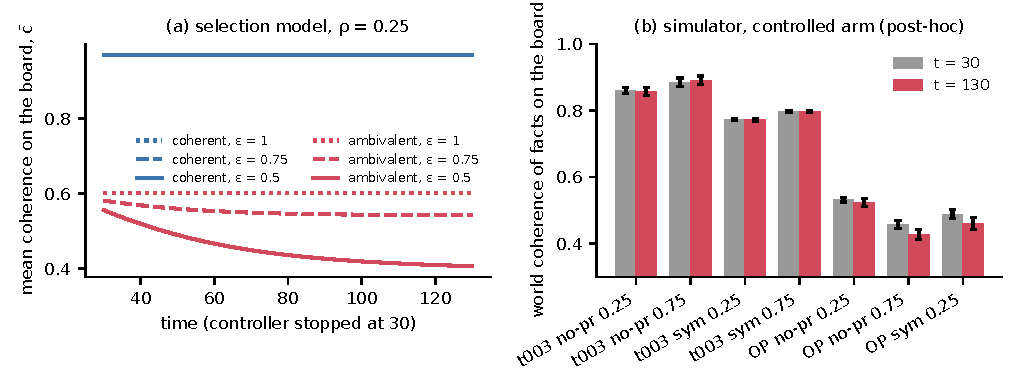
\includegraphics[width=\linewidth]{fig_selection.pdf}
\caption{\textbf{(a)} The selection model: mean coherence of controller facts on the board after the stop. With
ambivalent facts and vote-dependent reposting it falls; otherwise it stays. \textbf{(b)} Simulator: world coherence of
the controller facts on the board, at the stop and 100 time units later (95\% intervals; OP symmetric $\rho$ 0.75
omitted, because 83\% of its episodes have no controller post left).}
\label{fig:sel}
\end{figure}

\section{What this explains, and what it does not}
\begin{itemize}
\item \textbf{Explained, qualitatively:}
  \begin{itemize}
  \item why Object Placements fades while its exposure is constant;
  \item why its susceptibility falls;
  \item why task003 keeps its persuasive controller facts and Object Placements (no-proof, $\rho=0.75$) its least
    persuasive ones.
  \end{itemize}
  This gives level 2 of the common hierarchy, a changing strength mixture, a stated cause instead of an assumption.
\item \textbf{Not explained:}
  \begin{itemize}
  \item Object Placements no-proof at $\rho=0.25$: susceptibility falls 36\% with almost no selection. Strengths change
    at fixed facts, so a context effect remains there.
  \item The size of the fading at realistic $\varepsilon$.
  \item The flip under an $A2$ majority.
  \end{itemize}
\item \textbf{Not validated:} the parameter (coherence of the circulating facts) was found after seeing the data. It
  needs a setup not used to find it.
\end{itemize}

\paragraph{Reproducibility.}
\begin{itemize}
\item Today's code and results: \nolinkurl{analysis/theory_claude/fading_chain/} (start with \nolinkurl{results.md}).
\item Model code: \nolinkurl{phenomenological_fact_flow/fact_flow.py} and \nolinkurl{fading_chain/selection_model.py}.
\item Figures: \nolinkurl{make_figures.py} in this report's folder.
\end{itemize}

\end{document}
